\Chapter{Az alkalmazás felépítése}

% TODO: Le kell írni majd nagyvonalakban, hogy mik az alkalmazás fő részei és azok hogyan kapcsolódnak egymáshoz. Gyakorlatilag egy kliens-szerver-es ábrát kell csinálni, kiemelve rajta a sajátos megoldásokat.

% TODO: Itt lehet leírni azt is, hogy az egyes keretrendszerek és library-k választását mi indokolta. Annak kell érződnie, hogy minden funkcióhoz megfelelően lettek kiválasztva az eszközök. 

% TODO: Az API kialakításával kapcsolatos alapvető tudnivalókat is itt érdemes közölni. A részleteibe elég lesz majd csak az adott funkciókat bemutató fejezetekben belemenni.

\Section{Az alkalmazott technológiák bemutatása}

Egy webalkalmazás fejlesztése során különféle technológiák egyidejű használatára van szükség. A következő szakaszok ezek közül mutatják be a lényegesebbeket.

% TODO: Minden részhez kellenek majd olyan észrevételek, amelyekből rögtön látszik, hogy miért arra esett a választás, mi készült el vele, és úgy általában milyen módon kapcsolódik a dolgozat többi részéhez.

\SubSection{Python}

A Python egy általános célú programozási nyelv, támogatja az objektumorientált, a funkcionális, az imperatív és a procedurális programozási paradigmákat \cite{python}. Egy holland programozó, Guido van Rossum, kezdte el fejleszteni 1989-ben. 1991. február 20-án jelent meg. Az olvashatóság és a programozói munka megkönnyítése játszott kulcsszerepet a nyelv tervezése során. Interpreteres nyelv, tehát a forrás- és a tárgykód nem különül el. Ha írunk egy programot, az azonnal futtatható, ha van Python-értelmező a számítógépünkre telepítve. Széles körben használttá vált, hiszen platformfüggetlen és nagy számú kiegészítő könyvtár készült hozzá.

Egyetemi tanulmányaim során a legmélyebb ismereteket Java nyelvből szereztem, azonban szerettem volna még legalább egy nyelvet alaposabban megismerni. A Python mellett döntöttem, ami napjaink egyik legnépszerűbb programozási nyelvévé nőtte ki magát.

\SubSection{Flask}

Ahhoz, hogy webalkalmazást készíthessek, nem volt elegendő csupán a Python nyelv, szükséges volt egy webes keretrendszer használata is. Témavezetőm ajánlására a Flaskot választottam. A Flask egy Pythonban írt BSD licenccel rendelkező webes mikrokeretrendszer \cite{flask}. Nagyon jó választásnak bizonyult, hiszen egyszerű, minimalista, megfelelően dokumentált és rugalmasan bővíthető.

\SubSection{SQLAlchemy}

Az SQLAlchemy egy MIT licenccel rendelkező, nyílt forráskódú ORM rendszer Python nyelvhez \cite{sqlalchemy}. Alkalmas adatbázistáblák információnak kinyerésére, egyszerűbb és összetettebb lekérdezések generálására, adatbázis-manipulációs műveletek elvégzésére.

Sessionök végzik az adatbázis-műveleteket, amelyek alapja az ún. engine, ez az adatbázis-kapcsolatot reprezentálja. A táblákba való rekordbeszúrás úgy történik, hogy az általunk előre definiált osztályok attribútumainak értéket adunk, majd az adatbázishoz tartozó sessionbe beszúrjuk őket. A session a perzisztenciáért is felel, így már létező rekordot reprezentáló osztályon végzett módosítás akár azonnal megjelenhet az adatbázisban is.

Többek közt teljesítménye és használhatósága miatt jelenleg a legnépszerűbb ORM rendszer Python nyelvhez, így egyértelmű volt, hogy én is ezt fogom használni az alkalmazásom elkészítéséhez. 

\SubSection{HTML}

A HTML egy mozaikszó, melynek jelentése \textit{HyperText Markup Language}, vagyis hiperszöveges jelölőnyelv. Egy leírónyelv, weboldalak készítésére fejlesztették ki. A World Wide Web Consortium (W3C) támogatásával internetes szabvánnyá vált \cite{html}. Az állományok azokat a szimbólumokat tartalmazzák, amelyek leírják, hogy a böngészőnek milyen formában kell megjeleníteni, illetve feldolgozni az állomány tartalmát.

Legújabb verziója a HTML5, amelynek az egyik fő célja, hogy a webes alkalmazások használata különböző pluginek (pl. Adobe Flash, Microsoft Silverlight) telepítése nélkül is lehetséges legyen. Audio- és videofájlok beszúrására külön tageket hoztak létre (\texttt{<audio>}, \texttt{<video>}), illetve bevezettek egy ún. <canvas> taget. Ez tulajdonképpen egy rajzvászon, amelyre JavaScripttel tudunk rajzolni.

\SubSection{JavaScript}

A JavaScript legfőképp honlapok és webalkalmazások készítésére használt scriptnyelv, azonban webböngészőn kívüli környezetben is használják \cite{javascript}. A JavaScript szabványa az ECMAScript. 2012-től kezdődően mindegyik modern böngésző támogatja az ECMAScript 5.1.-et. Használatával a statikus weboldalak dinamikussá és interaktívvá tehetők. Az utasítások értelmezését a böngészőprogram végzi. Szerepelhet a HTML-fájlban vagy külön, \texttt{.js} kiterjesztésű szövegfájlban is. A HTML-dokumentumban \\ \texttt{<script>} tagek közé kell elhelyezni a JavaScript utasításokat.

\SubSection{AngularJS}

Az AngularJS egy nyílt forráskódú JavaScript keretrendszer, melyet a Google fejlesztett ki dinamikus webalkalmazások készítésére \cite{angularjs}. Rengeteg kiegészítő modul is elérhető hozzá, amik nagyban megkönnyíthetik a fejlesztést. Az Angular a manapság nagyon népszerű MVC (\textit{Model View Controller}) modellt használja. A HTML-fájlok a nézetek (view), és JavaScriptben íródnak a modellek és a kontrollerek.

Kétirányú adatkapcsolást alkalmaz, ami annyit tesz, hogy a nézetben bekövetkezett bárminemű változás azonnal tükröződik a modellben, illetve a modell változásai is a nézetben. Az alkalmazás üzleti logikáját a kontrollerek valósítják meg.

\SubSection{CSS}

A CSS a \textit{Cascading Style Sheets} rövidítése, amely egy stílusleíró nyelv, a HTML-oldalak megjelenését írja le \cite{css}. Nagy előnye, hogy lehetőségünk van egy stíluslapot rendelni az összes oldalunkhoz, így egy helyen megadhatjuk az elemek megjelenítését, ezáltal egységes megjelenést biztosítva az oldalunknak. Egy esetleges későbbi módosítást is csak egy helyen kell eszközölni, és annak hatása az összes, az adott stíluslappal rendelkező, oldalon megjelenik.

A szintaxisa nagyon egyszerű, a stíluslap a stílust leíró szabályok sora. Minden szabály szelektorból és deklarációs szakaszból áll. A deklarációs szakaszban kapcsos zárójelek közt deklarációk adhatók meg. Egy deklaráció a tulajdonság nevéből, egy kettőspontból, a tulajdonság értékéből, és végül egy pontosvesszőből áll.

\SubSection{Bootstrap}

A Bootstrap egy manapság nagyon népszerű, nyílt forráskódú CSS-keretrendszer. Segítségével egyszerűen készíthetünk látványos, reszponzív weboldalakat \cite{bootstrap}. A reszponzivitás abban nyilvánul meg, hogy az oldal taralma dinamikusan változik a megjelenítő eszköztől függően. Olvashatóságot, egyszerű navigációt biztosít akár monitorról, tabletről vagy mobiltelefonról használjuk az adott weboldalt.

A Bootstrap alapja egy rácsrendszer. Sorokból (\texttt{.row}) és oszlopokból (\texttt{.col}) épül fel, egy sor 12 oszlopból áll. A rácsrendszer egymásba ágyazható, egy sorban vagy oszlopban lehetőség van újabb sorokat és oszlopokat létrehozni.

Szinte az összes HTML-elemhez találhatunk a rendszerben formázást, amit az adott HTML-elem \texttt{class} attribútumával tudunk beállítani.

\SubSection{Git}

A Git egy nyílt forráskódú, elosztott verziókezelő rendszer \cite{git}. A verziókezelő rendszer segítségével láthatjuk, hogy ki, mit, mikor módosított, a módosításokhoz megjegyzéseket fűzhetünk. Képes visszaállítani egy fájl bármelyik korábbi állapotát.

Támogatja azt, hogy egy időben több fejlesztő dolgozhasson ugyan azon a feladaton. Minden fejlesztőnek külön helyi repository-ja lehet, melyből miután elvégezte a módosításokat, feltöltheti azokat a központi repository-ba. Így megoldható, hogy egy fájlon egyszerre akár több ember is dolgozzon, miközben elkerülhetőek az egymást való felülírások is. A központi repository tartalmát is bármikor lekérhetjük saját repository-nkba, így mindig az aktuális kódokkal dolgozhatunk.

\SubSection{GitHub}

A GitHub egy Git-alapú webes verziókezelő tárhelyszolgáltatás \cite{github}. A GitHub mára a legnépszerűbb közösségi fejlesztői szolgáltatássá vált, fejlett verziókezelési és kollaborációs megoldásokkal rendelkezik. Az alkalmazásom verziókövetésére a GitHubot használtam, több alkalommal is hasznos volt számomra, hogy visszatérhettem egy adott fájl előző változatára.

Az alkalmazás forráskódja az alábbi linken megtekinthető és letölthető:
\begin{center}
\url{https://github.com/GabiBlue/MEnetrend}
\end{center}

\Section{Az alkalmazás fő részei}

Az alkalmazás szerveroldalon a Python/Flask keretrendszert, kliensoldalon pedig An\-gu\-lar\-JS-t használ. A nyers GTFS-adatok feldolgozására és adatbázisba való betöltésére a GTFSDB csomagot használom. Az adatbázisból a lekérdezéseket az SQLAlcehmy ORM-en keresztül végzem. Létrehoztam egy menetrend nevű csomagot, ami tulajdonképpen egy wrapperként szolgál a GTFSDB felé. A wrapper egy alacsonyabb szintű programészre épülve magasabb szintű funkciókat valósít meg, elfedve a technikai részleteket, ezáltal egyszerűbbé téve azt. Az alkalmazás logikai felépítést szemlélteti \aref{fig:architecture}. ábra.

\begin{figure}[htb]
\centering
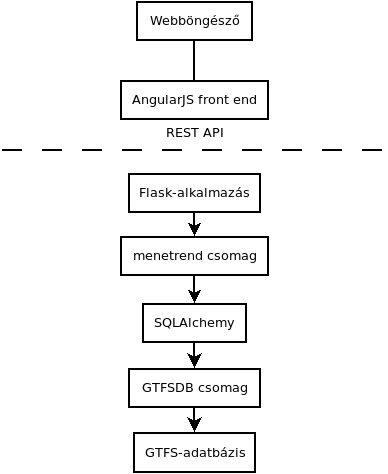
\includegraphics[scale=0.7]{kepek/architecture.png}
\caption{Az alkalmazás architektúrája}
\label{fig:architecture}
\end{figure}

A felhasználó egy böngészőn keresztül használja az alkalmazást. Ilyenkor az An\-gu\-lar\-JS-sel kialakított különböző nézeteket látja az alkalmazás használója. Az adatok a szerverről érkeznek, kliensoldalon az Angular kontrollerjei végzik a kérések elküldését a szerver irányába. A kapott válaszokat is a kontrollerek dolgozzák fel, biztosítják, hogy a kapott adatok a nézeteken megjelenjenek. A felhasználói felület a hatodik fejezetben kerül részletes bemutatásra.

Szerveroldalon egy többrétegű struktúrát alakítottam ki. A legalsó réteg maga az adatbázis. Ezt a GTFSDB nevű library segítségével hozom létre a nyers adatokból. Az adatbázisból való lekérdezéseket az SQLAlchemy-vel végzem. A GTFSDB csomagnak a lekérdezéseknél is szerepe van, hiszen a csomagban lévő \texttt{mapper} osztályokat használom. A GTFSDB-vel a negyedik fejezet foglalkozik részletesebben.

Az alkalmazás a Flask keretrendszert használja. A klienstől érkező kéréseket ez a réteg dolgozza fel. Ehhez, az esetleges paraméterellenőrzések után, az általam kialakított menetrend csomagot használja. A csomagban található metódusok kerülnek meghívásra, amelyek a már ismertetett, alsóbb rétegeket szólítják meg. A metódusok az így létrejött lekérdezések eredményeivel térnek vissza a flaskos rétegbe, amely pedig azokból előállítja a HTTP-válaszokat a kliens számára. Az adatok JSON-formátumban kerülnek továbbításra. A lekérdezések megfogalmazása történhetne a flaskos rétegben is, azonban előnyösebbnek véltem egy közbenső réteg bevezetését. A legnagyobb előnye a későbbi továbbfejleszthetőségben rejlik. A szerveroldali két felső réteg, a Flask és a menetrend csomag, bemutatása a hatodik fejezetben történik.
